\documentclass[12pt]{article}
\usepackage{graphicx}
\usepackage{booktabs}
\usepackage{longtable}
\usepackage{hyperref}
\usepackage[margin=1in]{geometry}
\usepackage{natbib}

\title{A Survey of Industrial Load Flexibility Rate Structures\\Across US RTOs and ISOs (2020--Present)}
\author{Draft prepared by EnergyRateFinder Agent}
\date{March 26, 2026}

\begin{document}

\maketitle

\begin{abstract}
Industrial load flexibility---the ability of large electricity consumers to adjust their consumption in response to grid conditions, price signals, or reliability events---is an increasingly important component of US wholesale electricity markets. This paper surveys the demand response and load flexibility rate structures and programs offered by the seven major Regional Transmission Organizations (RTOs) and Independent System Operators (ISOs) in the United States, focusing on developments from 2020 onwards. We document the market participation models, compensation mechanisms, and program designs across CAISO, PJM, ERCOT, MISO, ISO-NE, NYISO, and SPP, and discuss implications for industrial participants. In addition, the paper describes a companion GIS dashboard implementation that operationalizes the dataset through choropleth mapping, time-series visualization, typology-based program classification, and a sector-specific data center flexibility lens. The data center extension is motivated by the rapid growth of AI-oriented computing load, the mismatch between data center construction timelines and the slower pace of generation and transmission expansion, and the need to align digital infrastructure growth with grid decarbonization and reliability goals.
\end{abstract}

\section{Introduction}
The US electricity grid is undergoing a fundamental transformation driven by the growth of renewable energy, electrification of transportation and heating, and the emergence of new large loads such as data centers. In this context, demand-side flexibility---particularly from large industrial consumers---has become a critical resource for maintaining grid reliability and economic efficiency.

The growth of data centers adds urgency to this issue. In several states, data centers already represent a material share of total electricity demand, and the pace of new facility development is often faster than the timelines required to add new generation and transmission capacity. This creates a structural tension: the digital economy is expanding rapidly, but the physical power system is slower and more capital intensive to scale. At the same time, much of the existing generation fleet remains fossil-fuel-based, which raises concerns about the long-run environmental footprint of large computing loads.

This challenge also creates an opportunity. If data centers can participate as flexible, grid-interactive loads---rather than only as passive sources of demand growth---they could help absorb variable renewable generation, support reliability during stressed conditions, and reduce the need for the most carbon-intensive and expensive marginal resources. In that sense, the question is not simply whether data centers increase electricity demand, but whether they can be designed and operated in ways that make the broader power system more adaptable and more compatible with decarbonization.

Industrial load flexibility encompasses a range of actions: curtailing production during peak periods, shifting energy-intensive processes to off-peak hours, and providing ancillary services such as frequency regulation and operating reserves. RTOs and ISOs have developed a variety of programs and market mechanisms to compensate participants for providing these services.

This survey examines the rate structures and program designs across the seven US-based ISOs and RTOs, with a focus on the period from 2020 to the present. The seven grid operators collectively serve approximately two-thirds of total US electricity demand. A related objective of the present work is to connect these market structures to an implementation-oriented research agenda for flexible computing in AI data centers: one that can regulate power consumption in response to grid or aggregator requests while still respecting application constraints, quality-of-service objectives, and the operational realities of modern clustered computing systems.

\section{RTOs and ISOs in the United States}
The US electricity grid is managed by seven ISOs and RTOs operating within the continental United States:
\begin{itemize}
    \item \textbf{CAISO} -- California Independent System Operator (ISO)
    \item \textbf{NYISO} -- New York Independent System Operator (RTO)
    \item \textbf{ERCOT} -- Electric Reliability Council of Texas (ISO)
    \item \textbf{MISO} -- Midcontinent Independent System Operator (RTO)
    \item \textbf{ISO-NE} -- ISO New England (RTO)
    \item \textbf{SPP} -- Southwest Power Pool (RTO)
    \item \textbf{PJM} -- PJM Interconnection (RTO)
\end{itemize}

\noindent Regions outside these territories (notably the Southeast and Northwest) operate under bilateral market structures and are not covered in this survey.

\section{Rate Structures and Programs by RTO/ISO}

\subsection{California ISO (CAISO)}

CAISO offers several demand response market participation models that allow industrial loads to bid flexibility into the day-ahead, real-time, and ancillary services markets.

\subsubsection{Proxy Demand Resource (PDR)}
The Proxy Demand Resource model allows aggregations of end-use customers to participate in the wholesale energy market. PDRs submit bids to reduce load and are dispatched economically alongside supply resources. Key features include:
\begin{itemize}
    \item Compensation at the applicable Locational Marginal Price (LMP) for energy reductions
    \item Subject to the \textbf{Net Benefits Test}, a monthly price threshold established under FERC Order 745 that sets the minimum bid price for cost-effective demand response
    \item Can participate in day-ahead and real-time energy markets
    \item Eligible for ancillary services with appropriate telemetry and certification
\end{itemize}

\subsubsection{Reliability Demand Response Resource (RDRR)}
RDRRs are dispatched during system emergencies and reliability events. These resources are compensated at market-clearing prices when activated.

\subsubsection{Proxy Demand Resource -- Load Shift Resource (PDR-LSR)}
Introduced to accommodate flexible loads (e.g., storage-like behavior), PDR-LSRs can bid both load curtailment (paid from the net benefits test threshold up to the bid cap) and load consumption (from less than \$0 down to the bid floor). This model allows bidirectional load participation.

\subsubsection{California State Programs}
In addition to CAISO market programs, California state agencies have developed out-of-market demand flexibility programs:
\begin{itemize}
    \item \textbf{CPUC Emergency Load Reduction Program (ELRP)}: Compensates participants for load reductions during extreme weather events; payments at approximately \$1,000/MWh for verified reductions (2021--2025 program period).
    \item \textbf{CEC Demand Side Grid Support (DSGS)}: Pays distributed energy resources for providing incremental supply or load reduction during grid emergencies.
    \item \textbf{CPUC Demand Flexibility Rulemaking}: Ongoing proceeding to develop dynamic rate structures and market-informed demand automation via the MIDAS platform.
\end{itemize}

\subsection{PJM Interconnection}

PJM operates the largest wholesale electricity market in the US, covering 13 states and the District of Columbia. Its demand response programs are administered through Curtailment Service Providers (CSPs).

\subsubsection{Economic Demand Response}
Industrial customers can participate in the energy market by reducing load when wholesale prices exceed their offer price. Compensation is at the applicable LMP, subject to the net benefits test threshold. Resources can participate in both day-ahead and real-time markets.

\subsubsection{Capacity Market (Reliability Pricing Model -- RPM)}
Demand response resources can offer into PJM's Forward Capacity Market (RPM) as Capacity Performance resources, receiving capacity payments for committing to reduce load during performance assessment hours. Key rates include:
\begin{itemize}
    \item Capacity Performance clearing prices varied by Locational Deliverability Area (LDA); Base Residual Auction clearing prices have ranged from approximately \$50/MW-day to over \$269/MW-day in recent auctions (2020/21 through 2025/26 delivery years)
    \item Non-performance penalties apply: resources failing to deliver during performance assessment intervals face charges based on the Net Cost of New Entry (Net CONE) $\times$ Balancing Ratio
\end{itemize}

\subsubsection{Ancillary Services}
Demand response can provide Synchronized Reserves and Non-Synchronized Reserves in PJM, earning market-clearing reserve prices plus a make-whole payment if needed.

\subsubsection{Winter Storm Elliott (December 2022)}
The December 2022 winter event highlighted the importance of demand response in PJM. Over 8,000 MW of demand response was called upon during extreme cold conditions, leading to PJM undertaking reviews of resource performance and updated Capacity Performance rules.

\subsection{Electric Reliability Council of Texas (ERCOT)}

ERCOT operates an energy-only market (no capacity market), which shapes its demand response programs differently from other RTOs.

\subsubsection{Load Resource Participation in Ancillary Services}
Industrial loads (``Load Resources'') can qualify through a Qualified Scheduling Entity (QSE) to provide:
\begin{itemize}
    \item \textbf{Responsive Reserve Service (RRS)}: Loads that can be interrupted within 10 minutes; compensated at the Ancillary Services Market Clearing Price (MCPC)
    \item \textbf{Non-Spinning Reserve}: Loads available for curtailment within 30 minutes; compensated at MCPC
    \item \textbf{Regulation Service}: Loads with real-time telemetry capable of following dispatch signals; compensated at regulation MCPC
    \item Loads also participate in Security-Constrained Economic Dispatch (SCED) and are dispatched based on their offer curves at real-time Settlement Point Prices
\end{itemize}

\subsubsection{Emergency Response Service (ERS)}
ERS provides compensation to loads (and certain generators) that commit to reduce consumption during grid emergencies. Programs include:
\begin{itemize}
    \item \textbf{10-minute ERS}: Resources available within 10 minutes of deployment
    \item \textbf{30-minute ERS}: Resources available within 30 minutes
    \item Compensation through a competitive procurement process; clearing prices have varied seasonally, typically ranging from \$3--\$15/MW per hour of availability
\end{itemize}

\subsubsection{Voluntary Load Response}
Loads may contract with their Load Serving Entity to receive financial benefits for reducing energy usage in response to wholesale price signals. This is an indirect form of demand response that does not require ISO-level market registration.

\subsubsection{Real-Time Co-Optimization (Upcoming)}
ERCOT has been directed by the PUCT to implement real-time co-optimization of energy and ancillary services, which will further integrate demand-side resources into market clearing.

\subsection{Midcontinent Independent System Operator (MISO)}

MISO spans 15 US states and the Canadian province of Manitoba. Its demand response programs focus on both emergency and economic participation.

\subsubsection{Load Modifying Resources (LMRs)}
LMRs are demand response resources that commit to reduce load during emergency conditions. They provide capacity through MISO's Planning Resource Auction (PRA). Key features:
\begin{itemize}
    \item LMRs receive capacity credits and are counted toward the resource adequacy requirement
    \item PRA clearing prices have ranged from approximately \$5/MW-day to over \$236/MW-day (the 2022/23 auction for MISO Zone 2--7 cleared at the Cost of New Entry)
    \item LMRs must be available to curtail during MISO Maximum Generation Events
\end{itemize}

\subsubsection{Demand Response Resources (DRRs) -- Type I and Type II}
\begin{itemize}
    \item \textbf{Type I DRR}: Behind-the-meter generation that can be dispatched; compensated at LMP
    \item \textbf{Type II DRR}: Load curtailment resources; also compensated at LMP when dispatched economically
\end{itemize}

\subsubsection{Emergency Demand Response}
During Maximum Generation Events, MISO can call upon LMRs and Emergency Demand Response resources. Compensation is typically at the greater of LMP or \$3,500/MWh (the Value of Lost Load cap under certain emergency conditions).

\subsection{ISO New England (ISO-NE)}

ISO-NE serves the six New England states and has progressively integrated demand resources into its wholesale markets.

\subsubsection{Forward Capacity Market (FCM)}
Demand resources can participate in ISO-NE's Forward Capacity Auctions (FCAs), receiving capacity payments for committing to reduce load when called upon. Key parameters:
\begin{itemize}
    \item FCA clearing prices have ranged from approximately \$2.00/kW-month to \$3.98/kW-month for recent commitment periods (FCA 14 through FCA 19, covering 2023--2028)
    \item Performance payments and penalties apply through the Pay-for-Performance mechanism
    \item Resources must demonstrate capability through annual audits
\end{itemize}

\subsubsection{Price-Responsive Demand (PRD)}
Effective June 1, 2018, ISO-NE introduced the PRD participation model, which allows demand resources to be settled at the real-time LMP for load reductions below a baseline.

\subsubsection{Day-Ahead and Real-Time Energy Markets}
Demand resources with appropriate metering can participate in energy and reserve markets, receiving LMP-based compensation for dispatched reductions.

\subsubsection{Demand-Response Threshold Price}
ISO-NE publishes monthly Demand-Response Threshold Price reports (derived from the FERC Order 745 net benefits test), representing the minimum price at which demand response is cost-effective for the system.

\subsection{New York ISO (NYISO)}

NYISO operates both reliability-based and economic demand response programs.

\subsubsection{Special Case Resources (SCR) -- ICAP Program}
SCRs are demand-side resources enrolled in NYISO's Installed Capacity (ICAP) market. Key features:
\begin{itemize}
    \item SCRs receive monthly ICAP capacity payments for committing to reduce load during system emergencies
    \item ICAP Spot Market Auction prices in New York City zones have been among the highest in the US, ranging from approximately \$5/kW-month to over \$15/kW-month in recent years
    \item Resources must reduce to their Firm Service Level within 2 hours of notification
    \item Minimum reduction: 100 kW (individually or aggregated)
\end{itemize}

\subsubsection{Emergency Demand Response Program (EDRP)}
EDRP provides voluntary, event-based demand response compensation. Participants are paid the greater of \$500/MWh or the real-time zonal LMP for verified load reductions during NYISO-declared events.

\subsubsection{Distributed Energy Resource (DER) Aggregation}
Since 2020, NYISO has been implementing its DER participation model, which allows aggregations of distributed resources (including flexible loads) to participate in the energy, capacity, and ancillary services markets as economic resources at LMP-based compensation.

\subsection{Southwest Power Pool (SPP)}

SPP operates the Integrated Marketplace across 14 states and has been expanding its demand-side participation mechanisms.

\subsubsection{Demand Response in the Integrated Marketplace}
Demand response resources can participate in SPP's Day-Ahead and Real-Time markets by offering load curtailment at specified prices. Compensation is at the applicable LMP when dispatched.

\subsubsection{Block Demand Response}
SPP allows block demand response resources to offer fixed-quantity curtailments, useful for industrial loads that cannot partially curtail.

\subsubsection{Price-Adaptive Load (PAL)}
SPP has been exploring Price-Adaptive Load use cases (a March 2026 roundtable is scheduled), which would allow large, flexible loads to submit price-responsive demand curves into the market.

\subsubsection{Capacity and Resource Adequacy}
Demand response counts toward SPP's resource adequacy requirements under its planning reserve margin. Member utilities can use demand response to meet a portion of their capacity obligations.

\section{Comparative Summary}

Table~\ref{tab:comparison} summarizes the key load flexibility programs and compensation mechanisms across all seven US RTOs/ISOs.

\begin{longtable}{p{2cm}p{3.5cm}p{3.5cm}p{4cm}}
\caption{Comparison of Industrial Load Flexibility Programs Across US RTOs/ISOs}\label{tab:comparison}\\
\toprule
\textbf{RTO/ISO} & \textbf{Energy Market DR} & \textbf{Capacity/Reliability DR} & \textbf{Key Compensation Range} \\
\midrule
\endfirsthead
\toprule
\textbf{RTO/ISO} & \textbf{Energy Market DR} & \textbf{Capacity/Reliability DR} & \textbf{Key Compensation Range} \\
\midrule
\endhead
CAISO & PDR, PDR-LSR at LMP & RDRR; ELRP at \$1,000/MWh & LMP + state programs up to \$1,000/MWh \\
\midrule
PJM & Economic DR at LMP & Capacity Performance (RPM) & RPM: \$50--\$269+/MW-day \\
\midrule
ERCOT & SCED at Settlement Point Price & ERS (\$3--\$15/MW-hr); RRS at MCPC & Energy-only; AS MCPC varies \\
\midrule
MISO & DRR Type I/II at LMP & LMR via PRA & PRA: \$5--\$236/MW-day \\
\midrule
ISO-NE & PRD at LMP & FCM Pay-for-Performance & FCA: \$2--\$4/kW-month \\
\midrule
NYISO & DER at LMP & SCR ICAP; EDRP $\geq$\$500/MWh & ICAP: \$5--\$15+/kW-month \\
\midrule
SPP & Integrated Marketplace at LMP & Resource adequacy credit & LMP-based; capacity credit varies \\
\bottomrule
\end{longtable}

\section{Key Trends (2020--Present)}

Several notable trends have emerged across all RTOs/ISOs since 2020:

\begin{enumerate}
    \item \textbf{Performance-based compensation}: All RTOs have moved toward pay-for-performance designs that reward actual delivery and penalize non-performance during critical events, especially after Winter Storm Uri (2021, ERCOT) and Winter Storm Elliott (2022, PJM).

    \item \textbf{Integration of DERs and storage}: Markets are increasingly accommodating hybrid resources, bidirectional load participation (e.g., CAISO's PDR-LSR), and aggregated distributed energy resources (NYISO DER model).

    \item \textbf{Rising capacity prices}: Several markets have seen significant increases in capacity clearing prices, driven by resource retirements, growing demand from data centers, and tighter reserve margins. PJM's 2025/26 BRA clearing at record levels and MISO's 2022/23 auction spike are notable examples.

    \item \textbf{Large load integration}: ERCOT and CAISO have established dedicated processes for integrating large new loads (particularly data centers and crypto mining facilities), with ERCOT publishing specific guidelines for crypto mining facility participation in economic DR.

    \item \textbf{State-level programs}: California's ELRP, DSGS, and demand flexibility rulemaking represent a growing trend of state-level programs supplementing ISO market mechanisms.
\end{enumerate}

\section{Analysis and Machine Learning}

A classification model can be developed to identify patterns in the collected rate structures across the seven RTOs/ISOs. Potential features for such a model include:
\begin{itemize}
    \item Market type (energy-only vs. capacity + energy)
    \item Compensation mechanism (LMP-based, fixed rate, auction-based)
    \item Notification time requirement (10 min, 30 min, 2 hr)
    \item Minimum resource size (kW)
    \item Performance penalty structure (binary vs. graduated)
    \item Seasonal variation in rates
    \item Geographic zone pricing differentials
\end{itemize}

\noindent Clustering methods (e.g., k-means) and decision tree classifiers could be applied to categorize programs by their attractiveness to different industrial customer types (e.g., continuous process, batch process, data centers).

\section{Digital Platform and Dataset Extensions}

To make the comparative survey operational for practitioners, the underlying dataset has been extended into an interactive GIS dashboard. The dashboard includes polygon boundaries for the seven RTO/ISO footprints, region-level numeric rate summaries, program-level metadata, time-series histories for 2020--2025, and REST endpoints for local editing and export. This implementation transforms the survey from a static literature summary into an exploratory decision-support tool.

\subsection{Dashboard Capabilities}

The dashboard now supports the following functions:
\begin{itemize}
    \item \textbf{Choropleth mapping}: Regions can be colored by energy, capacity, emergency, or ancillary-service compensation ranges.
    \item \textbf{Comparison mode}: Users can compare multiple RTOs/ISOs side-by-side using bar charts and structured market summaries.
    \item \textbf{Trend analysis}: Time-series plots show representative energy, emergency, and capacity values from 2020 through 2025.
    \item \textbf{Editable data model}: A Flask API supports updating summary rates, numeric ranges, and individual program entries.
    \item \textbf{Exportability}: The dataset can be exported as JSON or CSV for downstream analysis.
\end{itemize}

\subsection{Typology-Based Classification}

The program schema has been expanded to include a three-dimensional typology intended to improve interpretation beyond raw posted prices:
\begin{itemize}
    \item \textbf{Economic}: captures the potential revenue upside and volatility of a program's compensation mechanism.
    \item \textbf{Flexibility}: captures the operational speed and strictness of the response required from the load.
    \item \textbf{Programmatic}: captures telemetry, baseline, aggregation, qualification, and settlement complexity.
\end{itemize}

Each program is scored on a 1--5 scale along these dimensions and also carries short labels and notes. This is a useful bridge between market design and facility decision-making because it separates gross compensation opportunity from operational feasibility and administrative burden.

\subsection{Data Center Flexibility Lens}

The latest extension adds an explicit sector profile for large data centers. Rather than assuming a special ``data center tariff,'' the model evaluates how a default battery-backed data center portfolio would perform across each market. The broader research motivation is to support a data center management framework that can (i) regulate power consumption in response to grid or market signals, (ii) coordinate interactions among data centers, aggregators, and power providers, and (iii) respect the characteristics of real computing systems and AI workloads, including parallel execution, job preemption, and performance-versus-accuracy tradeoffs. The current profile assumes a combination of UPS or battery flexibility, cooling-system flexibility, and limited standby generation support. It then estimates two outputs for each region:
\begin{enumerate}
    \item an overall \textbf{market fit score} based on economic attractiveness, flexibility compatibility, and programmatic burden; and
    \item a scenario-based \textbf{gross annual value range} derived from program compensation ranges, assumed flexible MW, and assumed annual participation hours.
\end{enumerate}

Conceptually, the sector score can be written as
\[
\text{Fit Score} = w_E E + w_F F + w_P P,
\]
where $E$ is the economic score, $F$ is the flexibility-fit score relative to data center response capability, and $P$ is the programmatic-fit score after accounting for tolerance to administrative complexity. The current implementation uses weights of approximately 0.40, 0.35, and 0.25 for these three terms, respectively.

The annual value estimate is scenario-based rather than deterministic, and is intended to provide directional insight:
\[
\text{Annual Value} \approx \sum_{k \in K} \left( r_k \times MW_k \times H_k \right),
\]
where $r_k$ is the relevant compensation rate for program category $k$, $MW_k$ is the portion of the data center portfolio assumed to be flexible for that category, and $H_k$ is the assumed annual participation duration. This framing is particularly relevant for data centers, where flexibility often comes from batteries, thermal storage, cooling optimization, and backup generation rather than curtailment of core compute load.

\subsection{FlexDC-Sim-Calibrated Regional Analysis}

To move beyond a purely heuristic lens, we calibrated the regional data center analysis with simulation outputs generated using the open-source FlexDC-Sim framework \citep{flexdc_sim}. A one-hour baseline run was executed using the reference low-utilization experiment setup with an AQA runtime policy and AI-inference workload mix. The resulting performance metrics were then used as a calibration layer over all RTO/ISO market valuations.

The simulation run produced a 90th-percentile tracking error of approximately 0.301, a job-type QoS violation ratio of approximately 0.75, and a mean execution slowdown of approximately 0.063. We convert these into a composite deliverability factor that scales scenario value estimates to reflect practical power-tracking and service-quality limits:
\[
\text{Deliverability} = 0.55(1-\epsilon_{90}) + 0.35(1-v_{qos}) + 0.10(1-s),
\]
where $\epsilon_{90}$ is the 90th-percentile tracking error, $v_{qos}$ is the job-type QoS violation ratio, and $s$ is mean execution slowdown. For this run, the derived deliverability factor is approximately 0.566.

Table~\ref{tab:flexdc_results} summarizes the resulting simulator-calibrated rankings and annual gross value ranges for a default data center flexibility portfolio across all seven US RTO/ISO regions.

\begin{longtable}{p{1.2cm}p{1.8cm}p{2.8cm}p{4cm}p{4.2cm}}
\caption{FlexDC-Sim-Calibrated Regional Data Center Flexibility Results}\label{tab:flexdc_results}\\
\toprule
\textbf{Rank} & \textbf{Region} & \textbf{Fit Score (1--5)} & \textbf{Estimated Annual Gross Value} & \textbf{Indicative Best Program Category} \\
\midrule
\endfirsthead
\toprule
\textbf{Rank} & \textbf{Region} & \textbf{Fit Score (1--5)} & \textbf{Estimated Annual Gross Value} & \textbf{Indicative Best Program Category} \\
\midrule
\endhead
1 & CAISO & 3.05 & \$4.1k--\$33.7k & Emergency-oriented participation (RDRR/ELRP class) \\
\midrule
2 & NYISO & 2.84 & \$67.4k--\$196.9k & Emergency and ICAP-linked participation \\
\midrule
3 & PJM & 2.79 & \$3.9k--\$22.0k & Capacity-linked participation (RPM class) \\
\midrule
4 & ERCOT & 2.70 & \$1.8k--\$7.7k & ERS and ancillary-oriented participation \\
\midrule
5 & MISO & 2.69 & \$4.0k--\$52.8k & Emergency plus PRA-linked participation \\
\midrule
6 & ISO-NE & 2.67 & \$26.8k--\$57.8k & Ancillary and FCM-linked participation \\
\midrule
7 & SPP & 2.00 & \$7.1k--\$39.8k & Capacity-credit plus day-ahead/real-time DR \\
\bottomrule
\end{longtable}

These values should be interpreted as screening-level estimates rather than audited forecasts. Their purpose is to compare relative opportunity under a common technical-operational constraint set, not to provide binding revenue projections for specific facilities.

\subsection{What Can a Data Center Earn by Region?}

Using the baseline calibrated scenario and the default 10 MW flexible portfolio assumption (battery + cooling + generator-enabled flexibility), Table~\ref{tab:earnings_region} reports estimated annual gross earnings by region. We report a low/high range and a midpoint for easier screening.

\begin{longtable}{p{1.6cm}p{2.2cm}p{3.4cm}p{3.2cm}p{3cm}}
\caption{Estimated Annual Data Center Gross Earnings by Region (Baseline Calibrated Scenario)}\label{tab:earnings_region}\\
\toprule
\textbf{Rank} & \textbf{Region} & \textbf{Annual Gross Range} & \textbf{Midpoint} & \textbf{Midpoint per MW-year} \\
\midrule
\endfirsthead
\toprule
\textbf{Rank} & \textbf{Region} & \textbf{Annual Gross Range} & \textbf{Midpoint} & \textbf{Midpoint per MW-year} \\
\midrule
\endhead
1 & NYISO & \$67.4k--\$196.9k & \$132.1k & \$13.2k/MW-year \\
\midrule
2 & ISO-NE & \$26.8k--\$57.8k & \$42.3k & \$4.2k/MW-year \\
\midrule
3 & MISO & \$4.0k--\$52.8k & \$28.4k & \$2.8k/MW-year \\
\midrule
4 & SPP & \$7.1k--\$39.8k & \$23.5k & \$2.3k/MW-year \\
\midrule
5 & CAISO & \$4.1k--\$33.7k & \$18.9k & \$1.9k/MW-year \\
\midrule
6 & PJM & \$3.9k--\$22.0k & \$13.0k & \$1.3k/MW-year \\
\midrule
7 & ERCOT & \$1.8k--\$7.7k & \$4.7k & \$0.47k/MW-year \\
\bottomrule
\end{longtable}

These estimates are most useful for regional screening and relative prioritization. Actual realized earnings will depend on telemetry readiness, aggregator strategy, event frequency, baseline methodology, and local interconnection and market participation constraints.

To test scenario sensitivity, we also ran a second NoDR-style configuration (high $P$ ratio and near-zero $R$). This reduced QoS violations but materially worsened tracking behavior under the FlexDC-Sim cost/signal setup. Table~\ref{tab:flexdc_scenarios} summarizes the resulting calibration inputs.

\begin{table}[h]
\centering
\caption{FlexDC-Sim Scenario Comparison Inputs}\label{tab:flexdc_scenarios}
\begin{tabular}{lccc}
\toprule
\textbf{Scenario} & \textbf{Tracking Error p90} & \textbf{QoS Violation Ratio} & \textbf{Deliverability Factor} \\
\midrule
Baseline AQA & 0.301 & 0.75 & 0.566 \\
NoDR-style AQA & very high (signal mismatch) & 0.00 & 0.445 \\
\bottomrule
\end{tabular}
\end{table}

Under this two-scenario comparison, the regional rank ordering remained stable, but calibrated gross annual value estimates in the NoDR-style scenario were approximately 21.3\% lower on average than the baseline calibrated case. This is consistent with the interpretation that for flexible AI-oriented data centers, preserving tracking capability is at least as important as minimizing direct QoS violations when the objective is market participation value capture.

\subsection{NAICS-Based Large-Load Shortlist Screening}

To extend the analysis beyond a single data center archetype, we constructed a 24-code large-load NAICS shortlist covering data centers, primary metals, chemicals, pulp and paper, transportation equipment, cold chain, and water/environmental infrastructure \citep{naics_census}. For each shortlisted NAICS code, we assign a representative facility load ($MW_{typ}$), a flexibility factor ($f_{flex}$), and a participation factor ($f_{part}$). We then compute an effective flexible load:
\[
MW_{eff} = MW_{typ} \times f_{flex} \times f_{part}.
\]

Regional earnings are estimated by multiplying $MW_{eff}$ by the calibrated regional midpoint value-per-MW from the baseline FlexDC-Sim scenario. This produces a screening-level annual midpoint earning estimate for each NAICS-region pair.

Table~\ref{tab:naics_top10} reports the top-10 opportunities from this shortlist by best-region annual midpoint value.

\begin{longtable}{p{0.9cm}p{1.6cm}p{4.8cm}p{1.8cm}p{1.8cm}p{2cm}p{2.3cm}}
\caption{Top-10 NAICS Large-Load Opportunities from Screening Analysis}\label{tab:naics_top10}\\
\toprule
\textbf{Rank} & \textbf{NAICS} & \textbf{Industry} & \textbf{Typical MW} & \textbf{Eff. Flex MW} & \textbf{Best Region} & \textbf{Annual Midpoint} \\
\midrule
\endfirsthead
\toprule
\textbf{Rank} & \textbf{NAICS} & \textbf{Industry} & \textbf{Typical MW} & \textbf{Eff. Flex MW} & \textbf{Best Region} & \textbf{Annual Midpoint} \\
\midrule
\endhead
1 & 518210 & Data Processing, Hosting, and Related Services & 20.0 & 10.50 & NYISO & \$138.7k \\
\midrule
2 & 336111 & Automobile Manufacturing & 18.0 & 6.14 & NYISO & \$81.1k \\
\midrule
3 & 331110 & Iron and Steel Mills and Ferroalloy Manufacturing & 30.0 & 6.00 & NYISO & \$79.3k \\
\midrule
4 & 325120 & Industrial Gas Manufacturing & 15.0 & 4.68 & NYISO & \$61.8k \\
\midrule
5 & 334413 & Semiconductor and Related Device Manufacturing & 18.0 & 4.46 & NYISO & \$58.9k \\
\midrule
6 & 322121 & Paper (except Newsprint) Mills & 16.0 & 4.38 & NYISO & \$57.8k \\
\midrule
7 & 322122 & Newsprint Mills & 14.0 & 4.06 & NYISO & \$53.6k \\
\midrule
8 & 324110 & Petroleum Refineries & 25.0 & 3.94 & NYISO & \$52.0k \\
\midrule
9 & 493120 & Refrigerated Warehousing and Storage & 8.0 & 3.64 & NYISO & \$48.1k \\
\midrule
10 & 327310 & Cement Manufacturing & 12.0 & 3.60 & NYISO & \$47.6k \\
\bottomrule
\end{longtable}

This shortlist is intentionally a screening instrument rather than a definitive ranking of all establishments. The key insight is that both (i) regional market economics and (ii) code-specific operational flexibility strongly shape expected value capture. The same NAICS code can materially shift rank under different regional price structures and participation constraints.

\subsection{Analysis Figures}

Figures~\ref{fig:regional_midpoint}--\ref{fig:naics_scatter} visualize the calibrated regional earnings and NAICS shortlist screening results.

\begin{figure}[htbp]
\centering
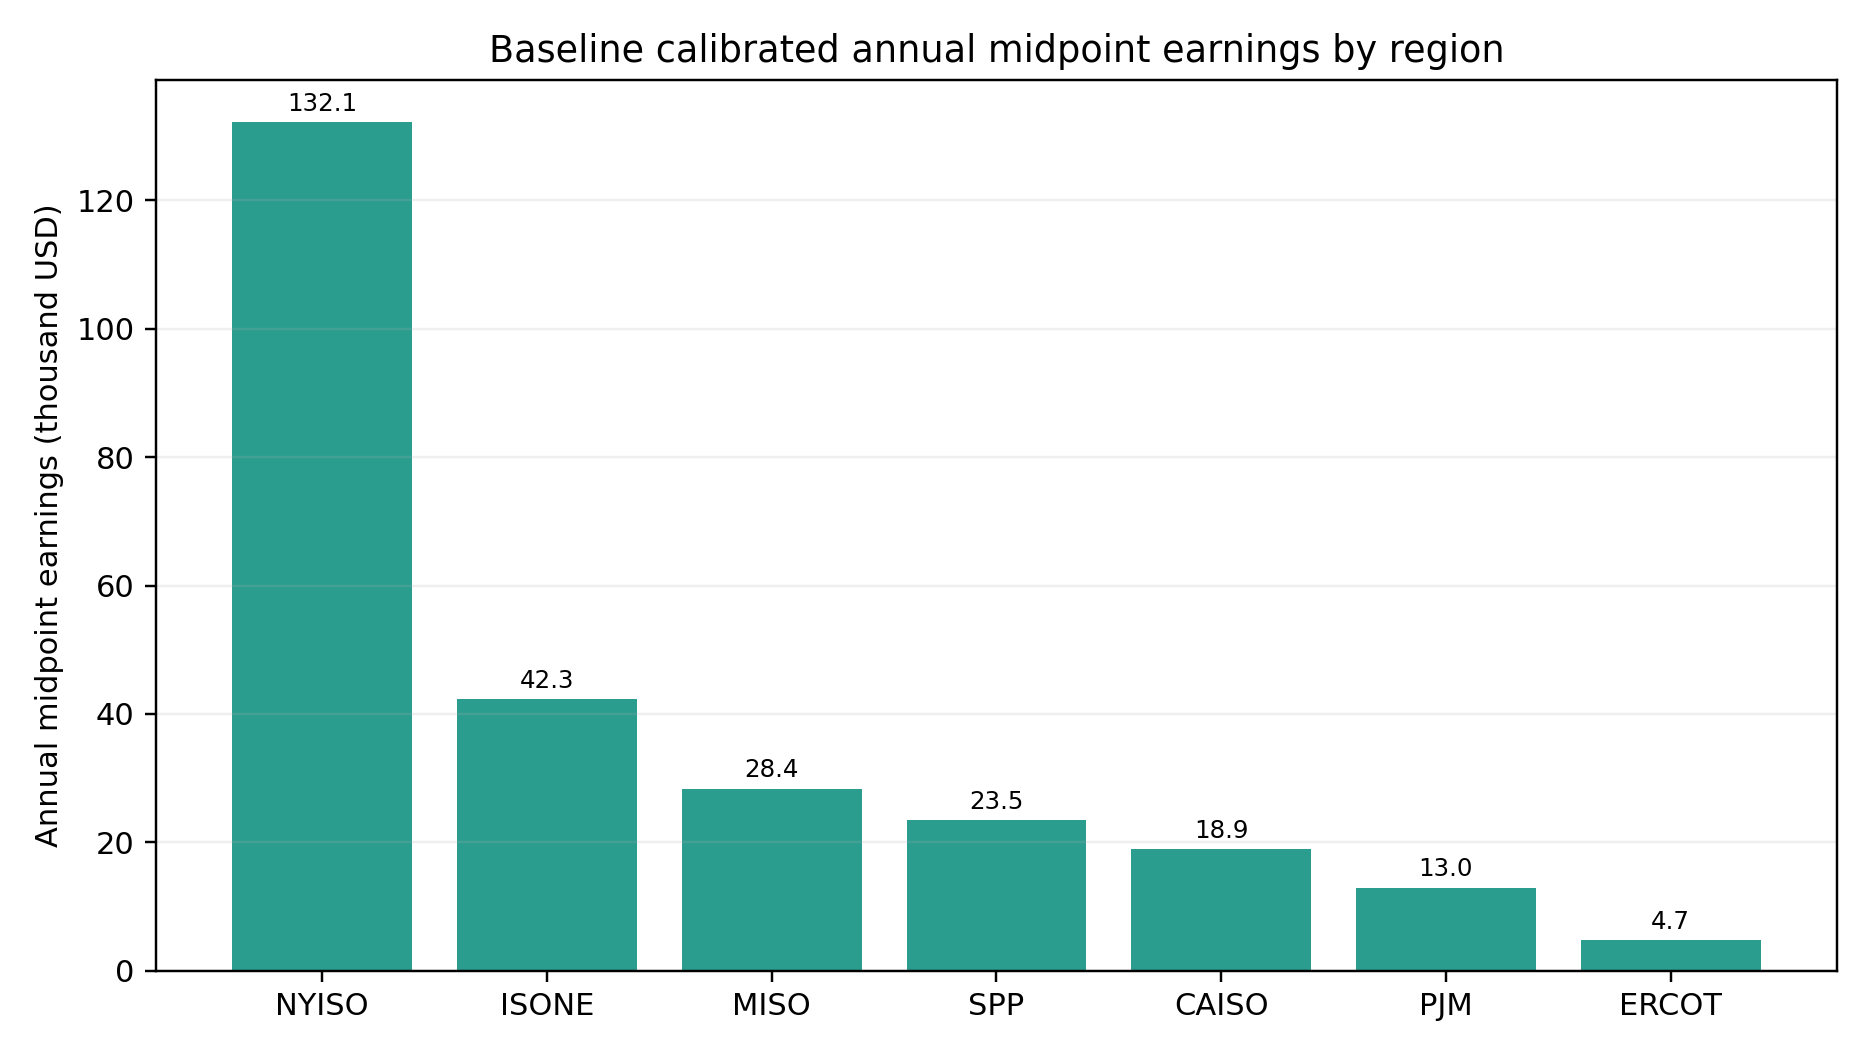
\includegraphics[width=0.92\linewidth]{analysis/figures/fig1_regional_midpoint_bar.png}
\caption{Baseline calibrated annual midpoint earnings by region.}
\label{fig:regional_midpoint}
\end{figure}

\begin{figure}[htbp]
\centering
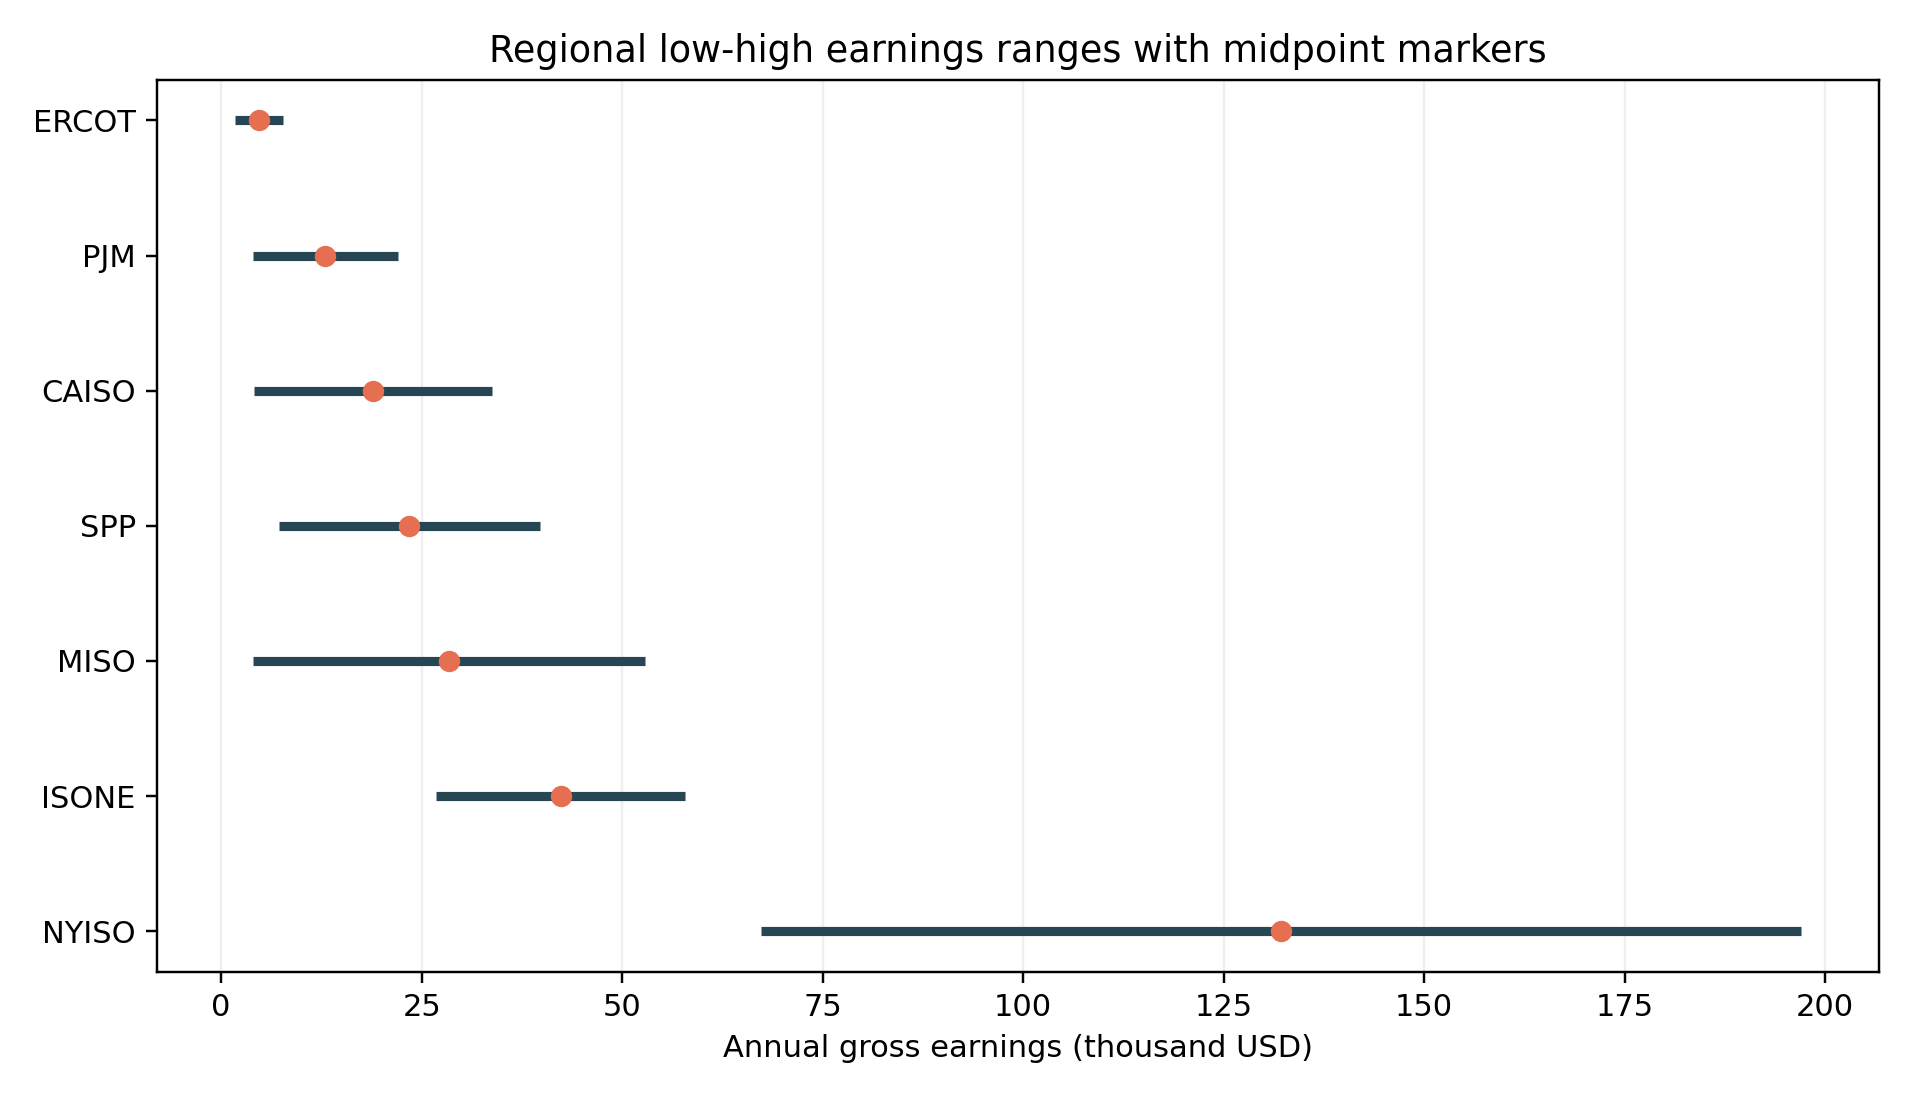
\includegraphics[width=0.92\linewidth]{analysis/figures/fig2_regional_range_lh.png}
\caption{Regional annual low-high earnings ranges with midpoint markers.}
\label{fig:regional_ranges}
\end{figure}

\begin{figure}[htbp]
\centering
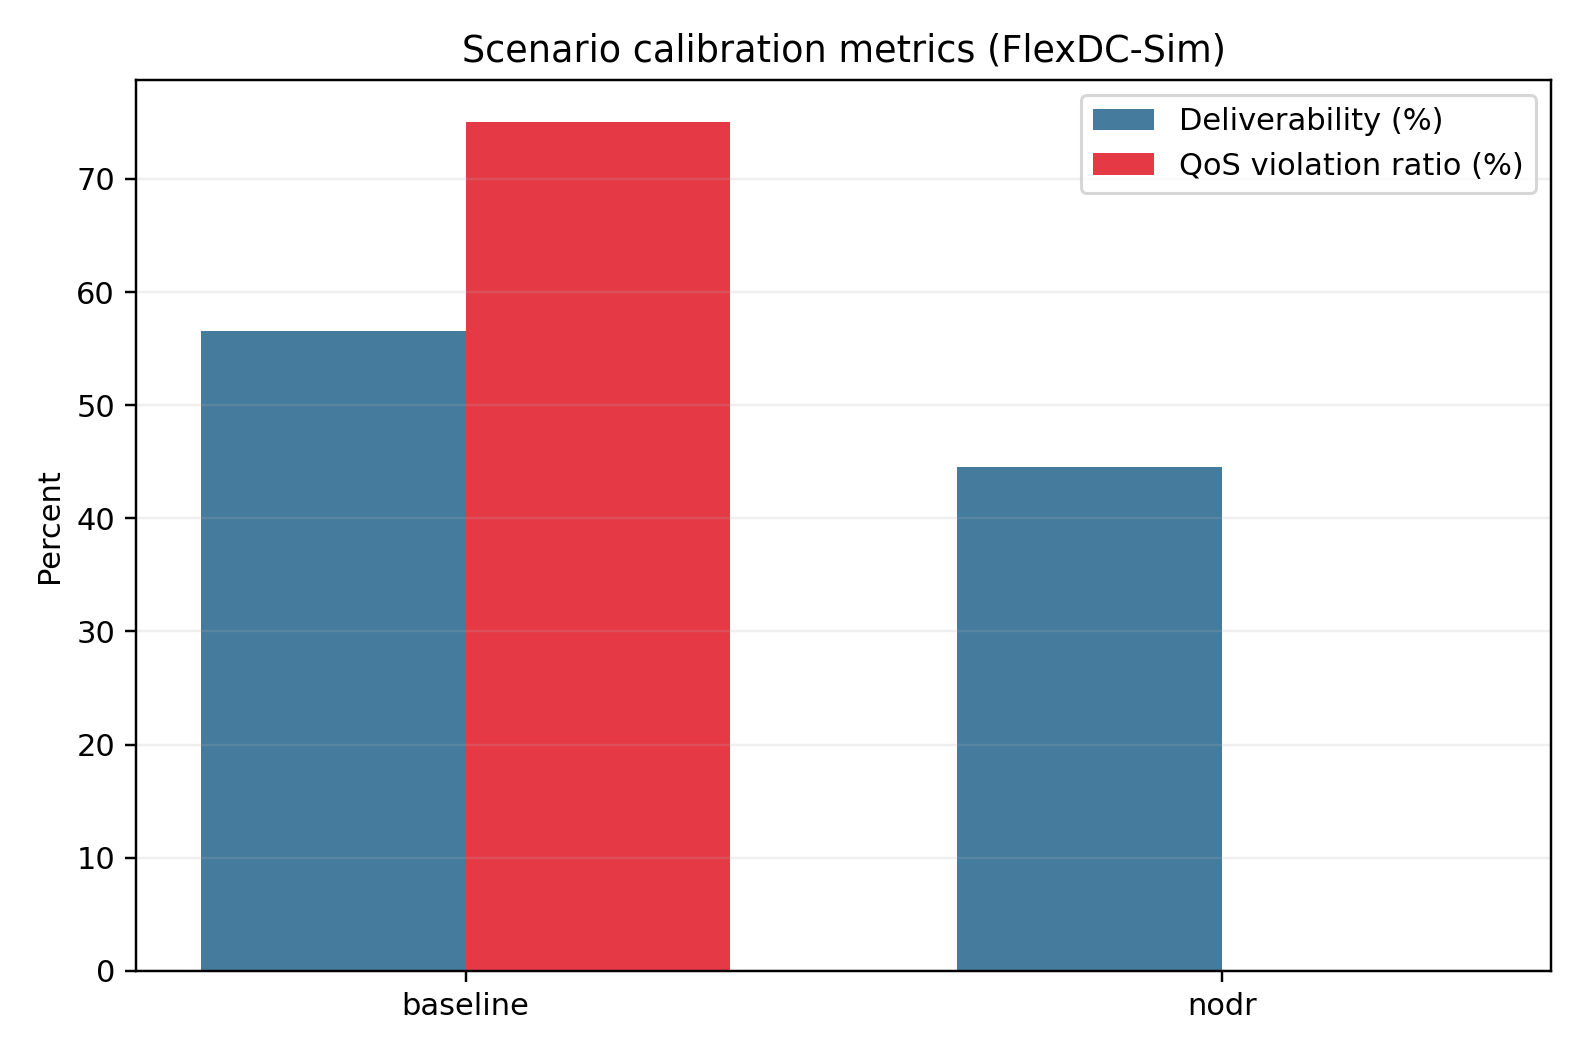
\includegraphics[width=0.84\linewidth]{analysis/figures/fig3_scenario_metrics.png}
\caption{FlexDC-Sim scenario calibration metrics (deliverability and QoS violation ratio).}
\label{fig:scenario_metrics}
\end{figure}

\begin{figure}[htbp]
\centering
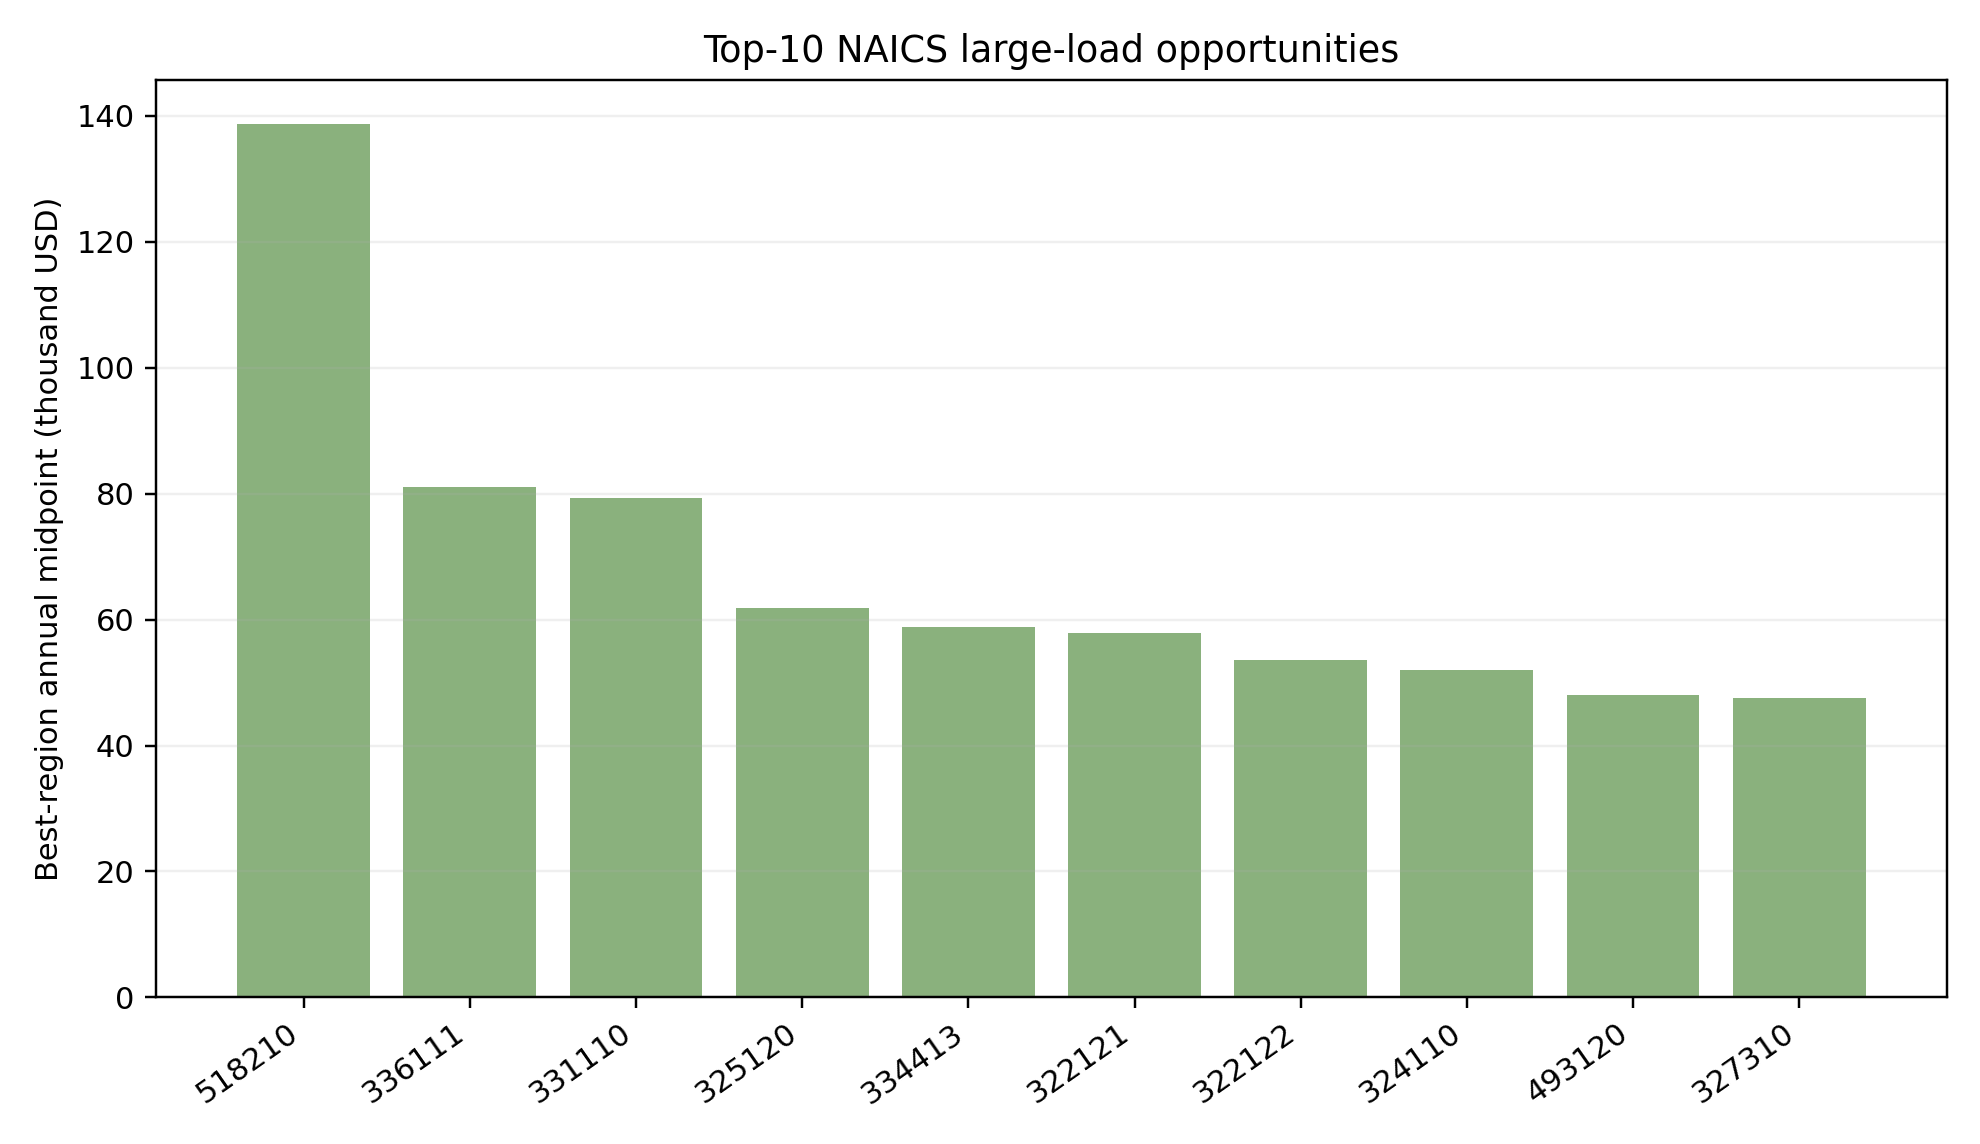
\includegraphics[width=0.96\linewidth]{analysis/figures/fig4_top10_naics.png}
\caption{Top-10 NAICS large-load opportunities by best-region annual midpoint estimate.}
\label{fig:top10_naics}
\end{figure}

\begin{figure}[htbp]
\centering
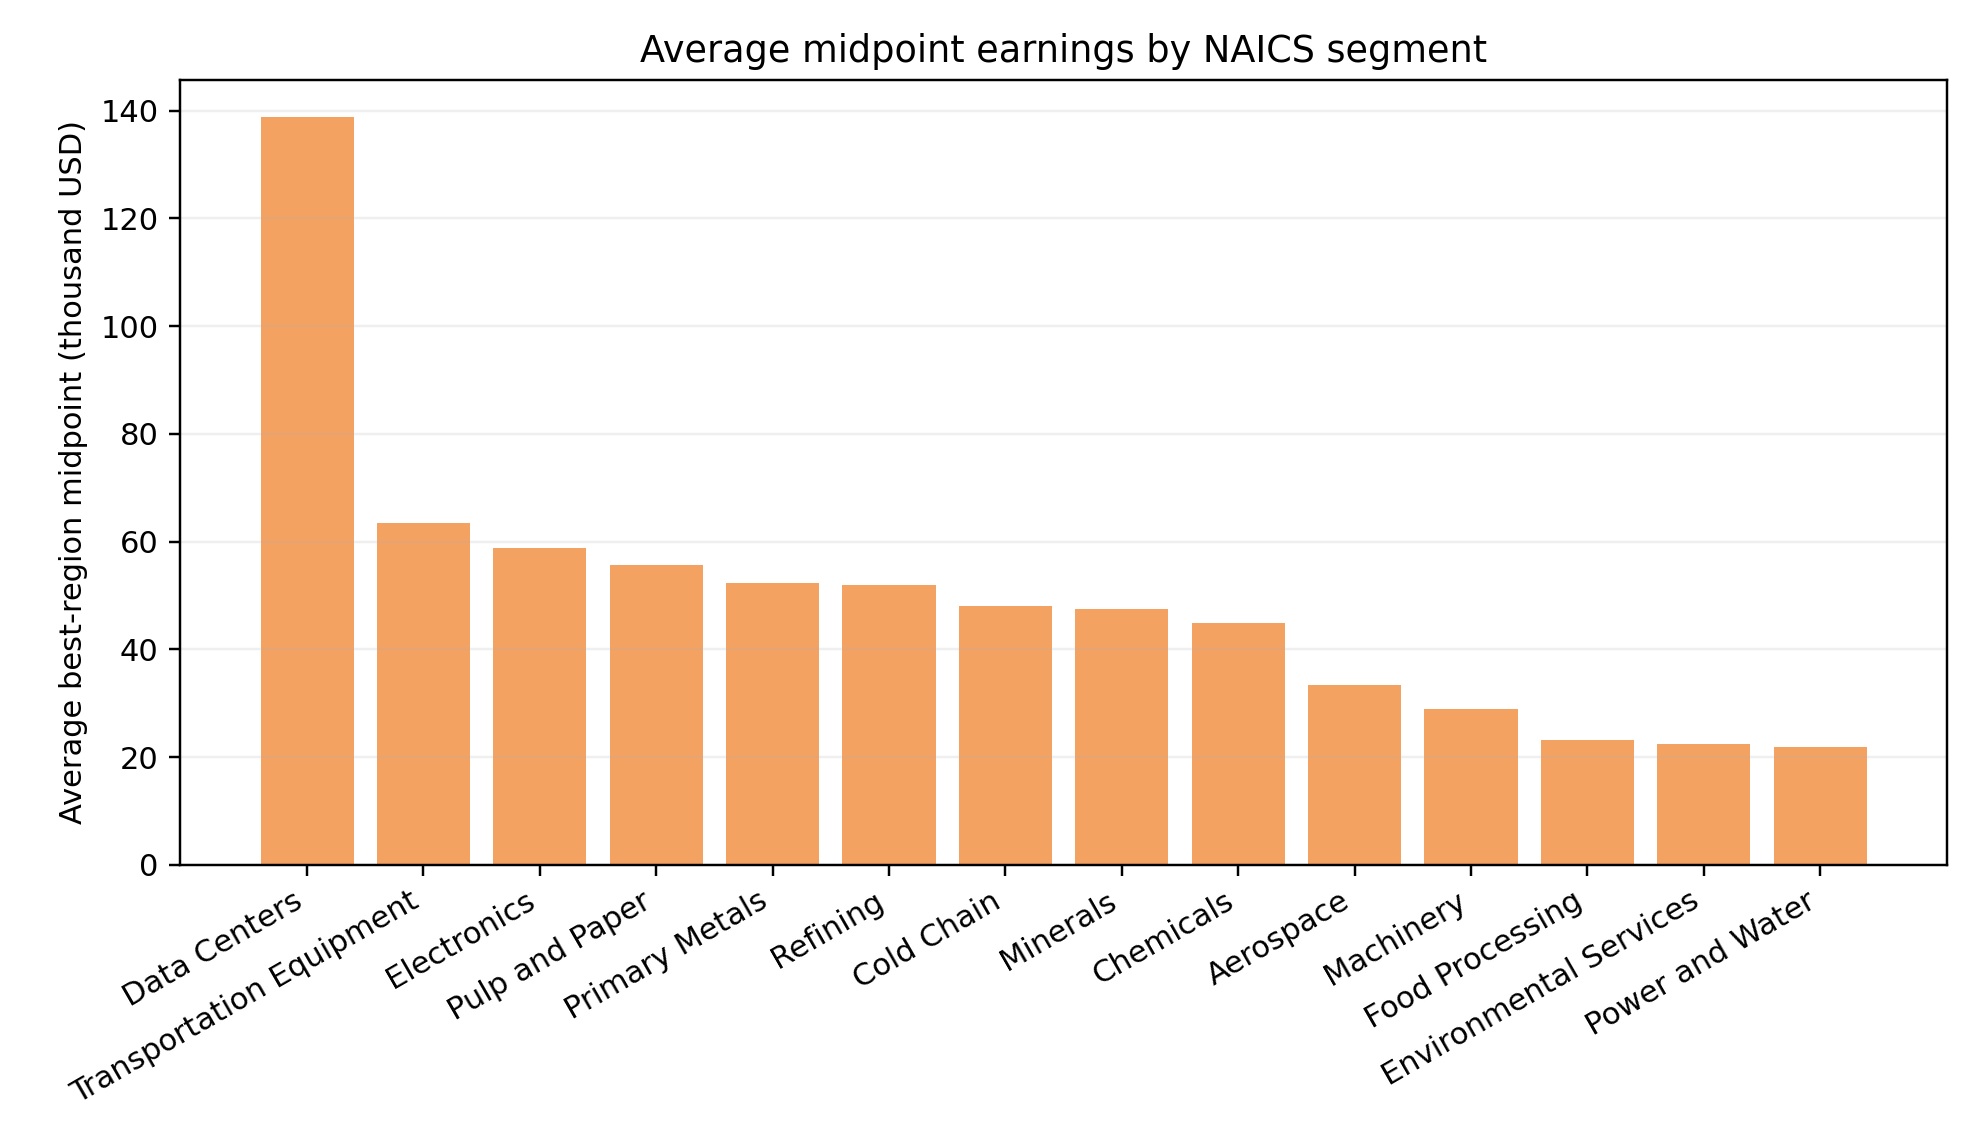
\includegraphics[width=0.96\linewidth]{analysis/figures/fig5_segment_avg.png}
\caption{Average best-region annual midpoint earnings by NAICS segment.}
\label{fig:segment_avg}
\end{figure}

\begin{figure}[htbp]
\centering
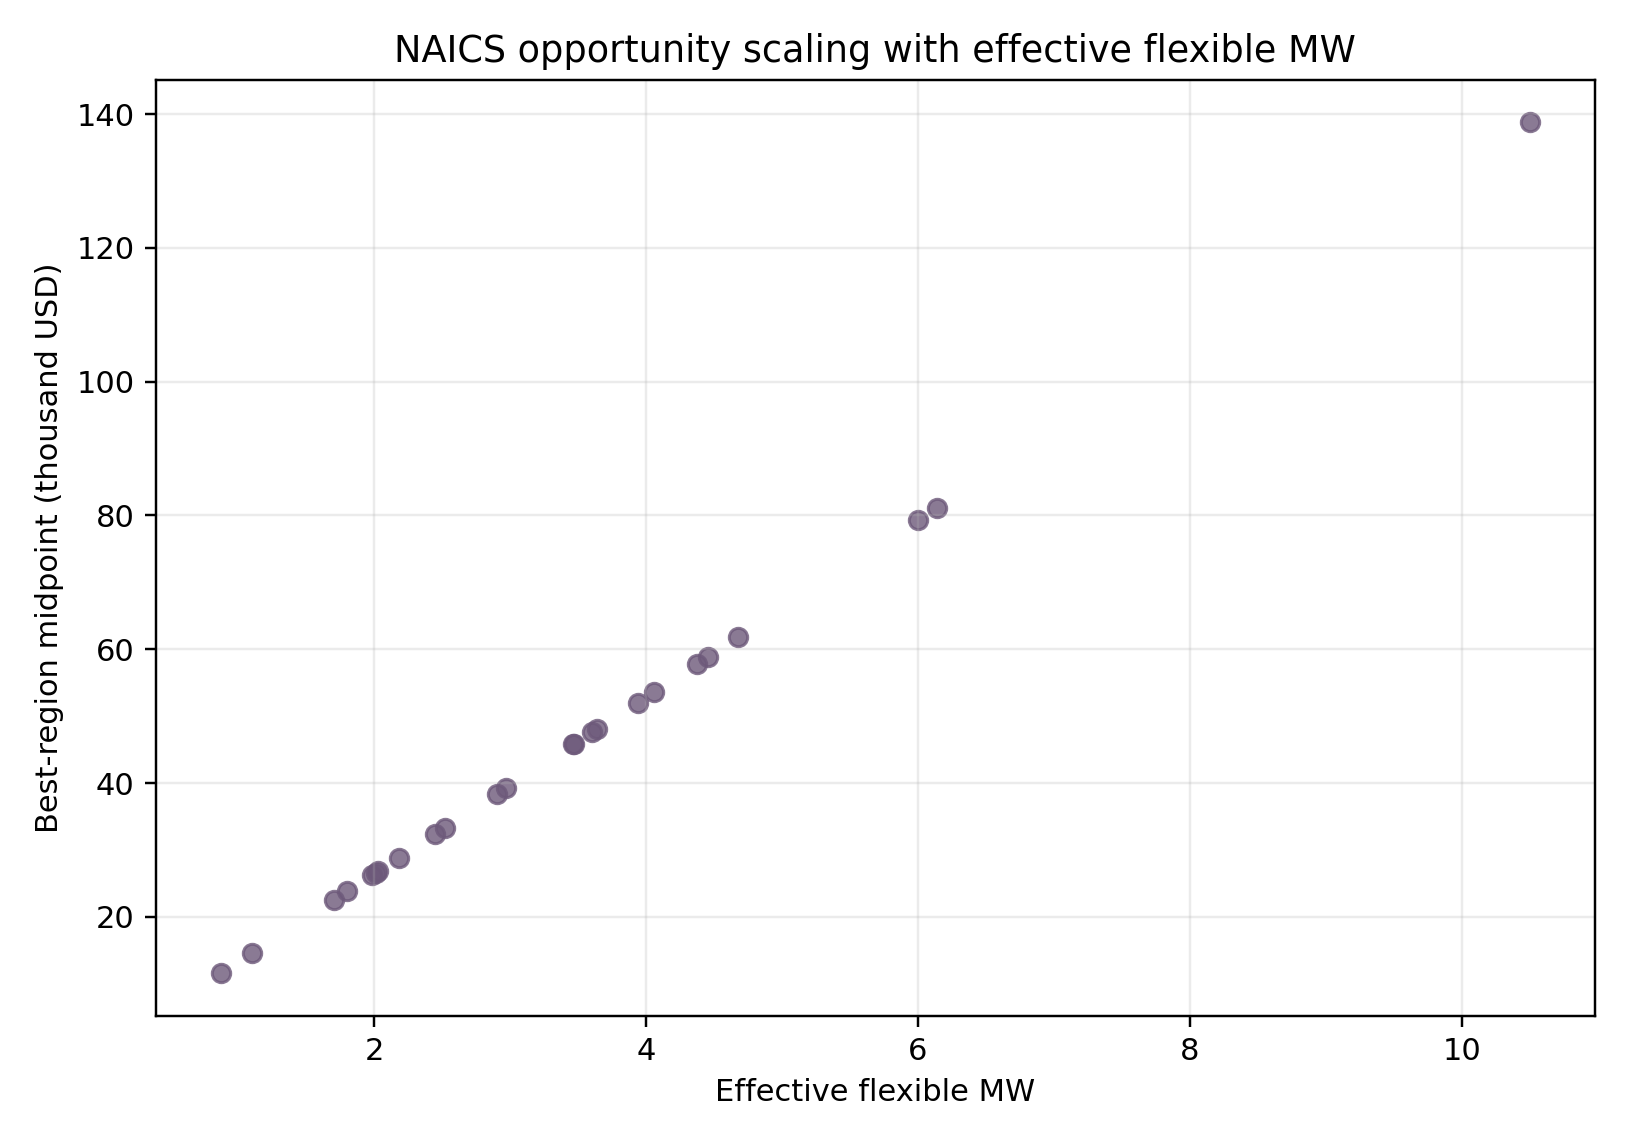
\includegraphics[width=0.86\linewidth]{analysis/figures/fig6_flexible_mw_scatter.png}
\caption{Scaling relationship between effective flexible MW and best-region annual midpoint earnings across shortlisted NAICS codes.}
\label{fig:naics_scatter}
\end{figure}

\subsection{Implications for Future Research}

These implementation updates make the dataset more suitable for sector-specific analysis. The same framework can be extended beyond data centers to industrial subsectors classified by NAICS code, including food processing, chemicals, paper, primary metals, refrigerated warehousing, and water-intensive industrial facilities. For data centers specifically, the next research step is to move from a stylized sector profile to a full operating framework that co-optimizes computational scheduling and grid participation under realistic constraints. The typology plus sector-profile approach therefore provides a structured path to evaluating not just ``what the market pays,'' but which facilities are operationally and administratively capable of capturing those payments while preserving service quality.

\section{Conclusion}

The landscape of industrial load flexibility rate structures across US RTOs and ISOs is diverse but converging on several common principles: LMP-based energy compensation, performance-linked capacity payments, and expanding participation models for distributed and aggregated resources. Since 2020, record capacity prices in PJM and MISO, emergency program activations following extreme weather events, and the integration of new large loads have all underscored the growing value of demand-side flexibility.

Industrial participants considering load flexibility should evaluate programs based on their operational characteristics (curtailment speed, duration, frequency tolerance), geographic location within an RTO/ISO, and the combination of energy, capacity, and ancillary service revenue streams available. The comparative data presented in this survey provides a starting framework for such analysis. The associated GIS platform and its typology- and sector-aware extensions show how this survey can be transformed into a practical analytical environment for market screening, program comparison, and large-load opportunity assessment.

\begin{thebibliography}{20}

\bibitem{ferc888} Federal Energy Regulatory Commission, ``Promoting Wholesale Competition Through Open Access Non-discriminatory Transmission Services by Public Utilities,'' Order No. 888, April 1996.

\bibitem{ferc745} Federal Energy Regulatory Commission, ``Demand Response Compensation in Organized Wholesale Energy Markets,'' Order No. 745, March 2011.

\bibitem{ferc2000} Federal Energy Regulatory Commission, ``Regional Transmission Organizations,'' Order No. 2000, December 1999.

\bibitem{caiso_dr} California ISO, ``Demand Response Market Participation Models,'' \url{https://www.caiso.com/generation-transmission/load/demand-response}, accessed March 2026.

\bibitem{pjm_dr} PJM Interconnection, ``Demand Response,'' \url{https://www.pjm.com/markets-and-operations/demand-response}, accessed March 2026.

\bibitem{ercot_dr} ERCOT, ``Demand Response Programs,'' \url{https://www.ercot.com/services/programs/load}, accessed March 2026.

\bibitem{miso_lmr} MISO, ``Resource Adequacy and Load Modifying Resources,'' \url{https://www.misoenergy.org/}, accessed March 2026.

\bibitem{isone_dr} ISO New England, ``Demand Resources,'' \url{https://www.iso-ne.com/markets-operations/markets/demand-resources}, accessed March 2026.

\bibitem{nyiso_dr} NYISO, ``Demand Response Programs,'' \url{https://www.nyiso.com/demand-response}, accessed March 2026.

\bibitem{spp_im} Southwest Power Pool, ``Integrated Marketplace,'' \url{https://www.spp.org/markets-operations/}, accessed March 2026.

\bibitem{wiki_rto} Wikipedia, ``Regional transmission organization (North America),'' \url{https://en.wikipedia.org/wiki/Regional_transmission_organization_(North_America)}, accessed March 2026.

\bibitem{flexdc_sim} S. G. Fernandes et al., ``FlexDC-Sim: An Open-Source Data Center Demand Response Simulator,'' GitHub repository, \url{https://github.com/sgfernandes/flexdc-sim}, accessed March 2026.

\bibitem{naics_census} U.S. Census Bureau, ``North American Industry Classification System (NAICS),'' \url{https://www.census.gov/naics/}, accessed March 2026.

\end{thebibliography}

\end{document}
